\documentclass[12pt]{article}
\usepackage{amsfonts, amsmath, amsthm, amssymb}
\usepackage[left=1cm,right=1cm,top=1cm,bottom=2cm]{geometry}
\usepackage{paralist}
\usepackage[T2A]{fontenc}
\usepackage[russian]{babel}
\usepackage[utf8]{inputenc}
\usepackage{graphicx}
\usepackage{wrapfig}

\usepackage{mathtools}
\usepackage{comment}
\DeclareGraphicsRule{*}{mps}{*}{}

\newcounter{problem}
\newcommand{\problem}{\par \bigskip \refstepcounter{problem}%
\textbf{№\arabic{problem}.} }

\def\avtor#1{\linebreak[2] \hspace*{\fill}{\small (\mbox{\textit{#1})}}}

\def \Problem#1{\par \bigskip \textbf{Problem №{#1}. }}
\def \solution{\par \bigskip \textbf{Solution. }}
\def \solutionI{\par \bigskip \textbf{First solution. }}
\def \solutionII{\par \bigskip \textbf{Second solution. }}
\def \solutionIII{\par \bigskip \textbf{Third solution. }}
\def \Lemma{\par \bigskip \textbf{Lemma. }}
\def \lemma#1{\par \bigskip \textbf{Lemma {#1}. }}
\def \proof{\par \bigskip \textbf{Proof. }}
\def \answer{\par \bigskip \textbf{Answer. }}
\def \marking{\par \bigskip \textbf{Marking scheme. }}
\def \corollary{\par \bigskip \textbf{Corollary. }}
\def\geq{\geqslant}
\def\leq{\leqslant}
\def\frac#1#2{\mathchoice{#1\over#2}{\hbox{\small$#1$}\over\mathstrut\hbox{\small$#2$}}{#1\over#2}{#1\over#2}} 

\begin{document}
\centerline{\sc \textbf{XXII Silk Road Mathematical Competition }}

\centerline{\sc \textbf{March 2023}}

\bigskip
\hrule
\bigskip

\textsl{\textbf{Attention!} 
Since the XXII Silk Road Mathematical Competition takes place in different countries on different dates, we ask you \textbf{not to disclose} these problems and not to discuss them publicly (especially through Internet) before May 25, 2023.}

\bigskip

\centerline{\sc \textbf{Solutions and marking schemes}}

\bigskip
\Problem{1} Point $M$ was chosen inside trapezoid $ABCD$ $(AD \parallel BC)$, and point $N$ was chosen inside triangle $BMC$ such that $AM \parallel CN$, $BM \parallel DN$. Prove that triangles $ABN$ and $CDM$ have equal areas. \avtor{Sedrakyan~N.}

\solution Let's prove the following lemma first.

\Lemma Points $N$ and $M$ are chosen on lateral sides $XY$ and $ZT$ of trapezoid $XYZT$, respectively. It is known that $XM \parallel ZN$. Then $YM \parallel TN$.

\proof Since 
$$
S_{NYZM}= S_{NYZ}+ S_{NZM}= S_{NYZ}+ S_{XNZ}= S_{XYZ} = S_{YZT}= S_{YZM}+ S_{YMT},
$$
then
$$
S_{YZM}+ S_{YMT}= S_{NYZM}= S_{YZM}+ S_{NYM},
$$
and thus $S_{YMT}= S_{NYM}$. So, $YM \parallel NT$. \qed

$$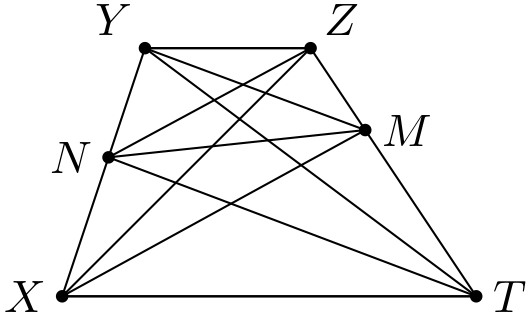
\includegraphics{img_1.jpg} \quad 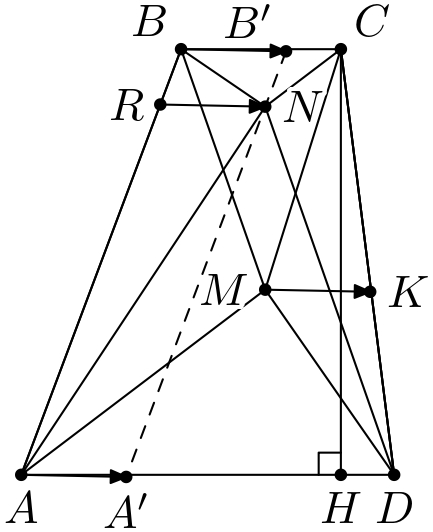
\includegraphics{img_2.jpg} $$

Let's return to the original problem. Let $R$ and $K$ be points on lines $BA$ and $CD$, respectively, such that $RN \parallel BC \parallel MK$. Let points $B’$ and $A’$ be the images of points $B$ and $A$, respectively, after parallel translation of the plane by vector $\overrightarrow{MK}$. 

Since $CN \parallel AM \parallel A’K$ and $DN \parallel BM \parallel B’K$, then $CN \parallel A’K$ and $DN \parallel B'K$. Let $CN$ intersect $B'A'$ at point $N'$. Since $A'K \parallel CN'$, then by applying the lemma to trapezoid $A'B'CD$ we get $B'K \parallel N'D$. Therefore, $DN \parallel B'K \parallel N'D$ and $N' = N$. This means that point $N$ lies on line $B’A’$. 

Hence,  $\overrightarrow{RN} =\overrightarrow{BB'}=\overrightarrow{MK}$. Let $CH$ be an altitude of triangle $CDA$. Then the distance between lines $BC$ and $DA$ is equal to $CH$ and
$$
S_{MCD}
=
\frac{1}{2} MK \cdot CD \cdot \sin \angle(MK,CD) 
=
\frac{1}{2} MK \cdot CD \cdot \sin \angle HDC 
=
\frac{1}{2} MK \cdot CH
.
$$
Similarly, $S_{BAN}=\frac{1}{2}RN \cdot CH$. Since $MK=RN$, then $S_{MCD}=S_{BAN}$, Q.E.D.

\marking

1. Proof of equality $S_{BCD}=S_{BCA}$ or equality $S_{BAD}=S_{CAD}$: \dotfill\textbf{1~point}

\smallskip

2. Proof of the lemma: \dotfill\textbf{2~points}

\smallskip

3. Proof of equality $\overrightarrow{RN} = \overrightarrow{MK}$: \dotfill\textbf{3~points}

\smallskip

\textit{For an incomplete computational solution (Cartesian or complex coordinates, vector or trigonometry calculus, etc.) points can only be awarded if the partial results of computations have been formulated in an equivalent form of the geometric statements mentioned in the scheme above.}


\Problem{2} Let $n$ be a positive integer. Each cell of a $2n\times 2n$ checkered square is painted in one of the $4n^2$ colors (some colors may be missing). We will call any two-cell rectangle in our square a \textit{domino}. We will also say that a domino is \textit{colorful} if its cells have different colors.

Let $k$ be the total number of colorful dominoes in our square. Let $\ell$ be the maximum integer such that every partition of the square into dominoes contains at least $\ell$ colorful dominoes. Determine the maximum possible value of $4\ell - k$ over all possible colorings of the square.  \avtor{Bogdanov~I.}

\answer $4n$.

\solution Consider a coloring of the square in which all cells are painted in pairwise different colors. In this coloring every domino is colorful, which means that $k = 2 \cdot 2n \cdot (2n - 1) = 8 n^2 - 4 n$ and $\ell = (2n)^2 / 2 = 2 n^2$. Hence, for this coloring we have $4 \ell - k = 4 n$.

It remains now to show that $4\ell-k\leq 4n$ for every coloring. For this purpose, consider four partitions into dominoes shown in the figure below. Partitions $\mathcal P_1$ and $\mathcal P_2$ consist respectively of horizontal rectangles only and of vertical rectangles only. Partition $\mathcal P_3$ has two columns, the leftmost and the rightmost, partitioned into vertical rectangles, and all other rectangles are horizontal. Partition $\mathcal P_4$ is obtained from $\mathcal P_3$ by rotation by $90^\circ$. 

\medskip
\centerline{\includegraphics{img_3.mps}}
\medskip

Note that any domino is present in at most two of the four partitions described above. Moreover, there are exactly $4n$ dominoes which are present in two of those partitions --- namely, vertical dominoes in $\mathcal P_3$ and horizontal dominoes in $\mathcal P_4$.

According to the problem statement, each of the four partitions described above contains at least $\ell$ colorful dominoes. However, there are only $k$ such dominoes in the square, and at most $4n$ of them appear in two partitions. Thus, $4 \ell \leq k + 4n \implies 4 \ell - k \leq 4n$.

\marking

1. Demonstration of a coloring for which $4 \ell - k = 4n$ and correct calculation of $k$ and $\ell$ \dotfill\textbf{1~point}

2. Proof of inequality $4 \ell - k \leq 4n$: \dotfill\textbf{6~points}


\Problem{3} Let $p$ be a prime number. Let's construct a directed graph on $p$ vertices, labeled with integers ranging from $0$ to $p - 1$. We draw an edge from vertex $x$ to vertex $y$ if and only if $y$ is equal to the remainder of division by $p$ of number $x^2 + 1$. Let $f(p)$ denote the length of the longest directed cycle in this graph. Prove that $f(p)$ can attain arbitrarily large values. \avtor{Zimanov~А.}

\solution Consider a sequence of non-negative integers $\{ a_n \}_{n = 0}^{\infty}$, defined as $a_0 = 0$ and $a_{n + 1} = a_{n}^2 + 1$ for all $n \geq 0$. For a positive integer $x$, define $d(x)$ as the set of its prime divisors. Let $S = \bigcup_{n = 1}^{\infty} d(a_n)$ be the set of all prime numbers which divide at least one of the positive elements of the sequence $\{ a_n \}$. Let's prove that $S$ is infinite. To do this, we prove the following lemma first:

\Lemma Let $n > m$ be non-negative integers such that there exists a prime number $p$ that divides both $a_n$ and $a_m$. Then $p$ must also divide $a_{\gcd(n, m)}$ where $\gcd(n, m)$ is the greatest common divisor of $n$ and $m$.

\proof Since $a_m \equiv 0 \equiv a_0 \pmod{p}$, then $a_{m + 1} \equiv a_{m}^2 + 1 \equiv 1 \equiv a_{1} \pmod{p}$. Thus, we can prove by induction on $k \geq 0$ that $a_{m + k} \equiv a_{k} \pmod{p}$. Hence, $0 \equiv a_{n} \equiv a_{m + (n - m)} \equiv a_{n - m} \pmod{p}$, i.e. $a_{n - m}$ is divisible by $p$. This, in turn, allows us to apply Euclidean algorithm on these indices $n$ and $m$, eventually obtaining that $p$ divides $a_{\gcd(n, m)}$
\qed

\corollary If $q$ is an arbitrary prime number, then $a_{q}$ is coprime with each of $a_1, a_2, \ldots, a_{q - 1}$, since for every $1 \leq k \leq q - 1$ we have that $\gcd(k, q) = 1$, thus, if a prime number $p$ divides both $a_q$ and $a_k$, then $p$ also divides $a_{\gcd(k, q)} = a_1 = 1$ --- a contradiction.

\medskip

Let $p_1 = 2, p_2 = 3, p_3 = 5, \ldots$ be the sequence of all prime numbers. Then all of the sets $d(a_{p_1}), d(a_{p_2}), d(a_{p_3}), \ldots$ are non-empty and pairwise disjoint, hence, the set $S$ is infinite.

Now let's return back to the initial problem. Let's fix an arbitrary positive integer $N$. Since $S$ is an infinite set, while the set $\bigcup_{n = 1}^{N} d(a_{n})$ of prime divisors of the first $N$ positive elements of the sequence is finite, there exists a prime number $p \in S$ such that $p$ doesn't divide any of $a_1, a_2, \ldots a_N$, but it divides $a_M$ for some $M > N$.

Consider the graph from the problem statement for this particular prime $p$. Note that the transition $a_n \to a_{n + 1}$ corresponds to the edge from vertex $a_n \pmod{p}$ to vertex $a_{n + 1} \pmod{p}$. Additionally, vertex $0$ lies on a simple directed cycle in this graph, because $a_M \equiv 0 \equiv a_0 \pmod{p}$. Since none of $a_1, a_2, \ldots, a_N$ is divisible by $p$, the length of this cycle must be at least $N + 1$. Thus, $f(p)$, as the length of the longest cycle, must be at least $N + 1$ too. As we fixed an arbitrary positive integer $N$ and proved the existence of such a prime number $p$ that $f(p) > N$, we have proved that $f(p)$ can attain arbitrarily large values.

\marking

1. The sequence $\{ a_n \}$ of integers (not modulo $p$) is considered:\dotfill\textbf{1~point}

2. The problem is reduced to proving the infiniteness of $S$:\dotfill\textbf{2~points}

3. The lemma, or at least the transition from $n$ and $m$ to $(n - m)$, is proved:\dotfill\textbf{2~points}


\Problem{4} Let $\mathcal{M} = \mathbb{Q}[x, y, z]$ be the set of three-variable polynomials with rational coefficients. Prove that for any non-zero polynomial $P \in \mathcal{M}$ there exist non-zero polynomials $Q, R \in \mathcal{M}$ such that
$$
R(x^2 y, y^2 z, z^2 x)
=
P(x, y, z) Q(x, y, z)
.
$$ \avtor{Navid Safaei}

\solution Let's prove the following lemma first.

\Lemma For any non-zero $P \in \mathcal{M}$ there exists non-zero $R \in \mathcal{M}$ such that $R(x^3, y, z)$ is divisible by $P(x, y, z)$.

\proof Let $n = \deg P$ and
$$
P(x, y, z)
=
\sum_{i = 0}^{n}
a_i x^i B_i(y, z)
\quad
(B_i \in \mathbb{Q}[y, z]),
$$
$$
A_j(x, y, z)
=
\sum_{\substack{0 \le i \le n \\ i \equiv j \pmod{3}}}
a_i x^i B_i(y, z)
\quad
(0 \le j \le 2)
.
$$

Consider the following polynomial
$$
A_0^3 + A_1^3 + A_2^3 - 3 A_0 A_1 A_2 \not\equiv 0
.
$$
On one hand, since the degree of variable $x$ in each of its monomials is divisible by 3, then for some $R \in \mathcal{M}$ it is equal to $R(x^3, y, z)$. On the other hand,
$$
A_0^3 + A_1^3 + A_2^3 - 3 A_0 A_1 A_2 
=
(A_0 + A_1 + A_2)
(A_0^2 + A_1^2 + A_2^2 - A_0 A_1 - A_1 A_2 - A_2 A_0)
=
$$
$$
=
P (A_0^2 + A_1^2 + A_2^2 - A_0 A_1 - A_1 A_2 - A_2 A_0)
,
$$
i.e. $R(x^3, y, z)$ is divisible by $P(x, y, z)$. The lemma is proved.
\qed

\corollary For any non-zero $P \in \mathcal{M}$ and any non-negative integers $k, t, \ell$ there exists non-zero $R \in \mathcal{M}$ such that $R(x^{3^k}, y^{3^t}, z^{3^\ell})$ is divisible by $P(x, y, z)$. It can be easily proved by induction using the lemma in the induction step.

\medskip

Let's return to the original problem. Corollary, in particular, states that there exists $S \in \mathcal{M}$ such that $S(x^9, y^9, z^9)$ is divisible by $P(x, y, z)$. Let $n = \deg S$. Consider polynomial
$$
(xyz)^{6n} S(x^9, y^9, z^9) \not \equiv 0
.
$$
Each of its monomials is of the form
$$
\alpha (xyz)^{6n} x^{9a} y^{9b} z^{9c}
=
\alpha 
(xyz)^{6 (n - a - b - c)}
(xyz)^{6 (a + b + c)}
x^{9a} y^{9b} z^{9c}
=
$$
$$
=
\alpha 
(xyz)^{6 (n - a - b - c)}
(xyz)^{6 (a + b + c)}
x^{9a} y^{9b} z^{9c}
=
$$
$$
=
\alpha 
(xyz)^{6 (n - a - b - c)}
(x^2y)^{6a+3b}(y^2z)^{6b+3c}(z^2x)^{6c+3a}
=
$$
$$
=
\alpha
(x^2y)^{6a+3b + 2 (n - a - b - c)}
(y^2z)^{6b+3c + 2 (n - a - b - c)}
(z^2x)^{6c+3a + 2 (n - a - b - c)}
.
$$
Thus, there exists $R \in \mathcal{M}$ such that
$$
R(x^2 y, y^2 z, z^2 x)
=
(xyz)^{6n} S(x^9, y^9, z^9)
.
$$
Since $S(x^9, y^9, z^9)$ is divisible by $P(x, y, z)$, then $R(x^2 y, y^2 z, z^2 x)$ is also divisible by $P(x, y, z)$.

\par
\bigskip
\textbf{Comment.} The lemma can be proved in another way. Let $\omega = e^{\frac{2 \pi i}{3}}$ (primitive root of unity of the third degree) and
$$
H(x, y, z)
=
P(x, y, z) P(\omega x, y, z) P(\omega^2 x, y, z)
.
$$
Since $\overline{\omega} = \omega^2$, then for any $x, y, z \in \mathbb{R}$, 
$$
\overline{P(\omega x, y, z)}
=
P(\overline{\omega} x, y, z)
=
P(\omega^2 x, y, z)
\implies
$$
$$
\implies
\overline{H(x, y, z)}
=
H(x, y, z)
.
$$
It can be shown that $H$ has real (and rational) coefficients (we leave this as an exercise). Let $m = \deg H$ and
$$
H(x, y, z)
=
\sum_{i = 0}^{m}
h_i x^i C_i(y, z)
\quad
(C_i \in \mathbb{Q}[y, z]),
$$
$$
D_j(x, y, z)
=
\sum_{\substack{0 \le i \le n \\ i \equiv j \pmod{3}}}
h_i x^i C_i(y, z)
\quad
(0 \le j \le 2)
.
$$
Note that
$$
H(x, y, z)
=
H(\omega x, y, z)
=
H(\omega^2 x, y, z)
\implies
$$
$$
\implies
D_0 + D_1 + D_2
=
D_0 + \omega D_1 + \omega^2 D_2
=
D_0 + \omega^2 D_1 + \omega D_2
\implies
$$
$$
\implies
D_1
=
D_2
=
0
\implies
H = D_0
.
$$
Therefore, for some $R \in \mathcal{M}$,
$$
R(x^3, y, z)
=
H(x, y, z)
.
$$

Let 
$$
Q(x, y, z) 
=
P(\omega x, y, z) P(\omega^2 x, y, z)
.
$$
It can be shown that $Q \in \mathcal{M}$. Since
$$
R(x^3, y, z)
=
H(x, y, z)
=
P(x, y, z) Q(x, y, z)
,
$$
then $R(x^3, y, z)$ is divisible by $P(x, y, z)$.

\marking

1. Formulation of the lemma or of a special case of the corollary (considering only one-variable polynomials is acceptable) $\dotfill$ \textbf{1 point}

\smallskip

2. Proof of the fact that it is enough to consider only those $P$ that can be represented as $T(x^9, y^9, z^9)$, $T \in \mathcal{M}$ (in the solution above, for example, polynomial $P$ was replaced with polynomial $S(x^9, y^9, z^9)$ that is divisible by $P$). $\dotfill$ \textbf{5 points}

\smallskip

3. Solution of the problem for such $P$ that can be represented as $T(x^9, y^9, z^9)$, $T \in \mathcal{M}$. $\dotfill$ \textbf{1 point}

\smallskip

All points are additive.

\end{document}
